\section{Modelado de redes}
Muchas de las propiedades macroscópicas de los cuerpos se pueden entender en función de la estructura microscópica\parencite{Jacobs1997}\parencite{Garboczi1985}\parencite{Guyon1990} de los materiales. Por ejemplo, la resistencia macroscópica depende del agregado de  resistencias microscópicas a la deformación. Usualmente lo que se estudia son corpúsculos, dependiendo de la escala a la que se haga el estudio pueden ser átomos, radicales u objetos, que se unen para formar un cuerpo con secciones rígidas o blandas. Al estudio y caracterización de la rigidez de estas secciones se le conoce como \emph{percolación de rigidez}.

Específicamente con respecto a las proteínas, hace décadas que se conoce que la flexibilidad de los diferentes segmentos de una proteína es la que vincula su estructura con su función biológica\parencite{Gerstein1994}.

Para estudiar la rigidez de los cuerpos existen dos métodos principales: experimentalmente y mediante modelado computacional. Para la primera se utilizan diferentes técnicas de cristalografía de rayos X o mediante resonancia magnética nuclear. Un ejemplo de uso de rayos X para inferir la forma de una molécula se presenta en la figura \ref{fig:dna}, la cual presenta la imagen que permitió deducir la forma en espiral del ADN obtenida mediante técnicas de cristalográfica desarrolladas por Rosalind Franklin y por trabajos de Aaron Klug.

\begin{figure}
\center
\includegraphics[width=70mm]{./images/adn}
\caption{Imágen obtenida mediante cristalografía de rayos X que demuestra la forma en espiral del ADN}
\label{fig:dna}
\end{figure}

El modelado computacional, por otra parte, presentan los siguientes tres paradigmas en general:\parencite{Ahmed2013}

\begin{enumerate}
\item Homología: en el que se identifican regiones similares a otras regiones cuyo comportamiento ya se conoce.
\item Reconocimiento de plegado: en la que se identifican las formas en que se pliegan las proteínas mediante su analogía con otros métodos.
\item \emph{Ab initio}: en la que se predice el comportamiento de la molécula solamente conociendo una descripción de los átomos que la componen. Mediante algoritmos especializados se encuentran las regiones rígidas y flexibles de las redes.
\end{enumerate}

El presente trabajo se centra únicamente en procesos del modelado \emph{Ab Initio}. Específicamente en los algoritmos PG y VPG. Estos predicen únicamente mediante una lista de los átomos que componen una red o proteína las partes rígidas y las partes flexibles mediante el uso de conteo de restricciones.

\section{Modelado mediante conteo de restricciones}
El modelado de estructuras mediante el conteo de restricciones consiste en representar el cuerpo a modelar mediante cuerpos más pequeños que se interconectan para formar un cuerpo más grande. Las conexiones mantienen a la estructura unida pero tienen un costo en grados de libertad para los nodos individuales. Es decir, para mantenerse unidas se pierde cierta cantidad de movimiento o rotación. La cantidad de grados que queda en cada nodo representa la rigidez o la flexibilidad del cuerpo.

La percolación es un problema complejo inherentemente no local, es decir, para determinar las propiedades de una región dada, se debe examinar detalles estructurales que se encuentran lejos de la zona. Estos detalles dificultaban significativamente la implementación de un algoritmo eficiente. Los primero intentos tenían tiempos de corrida que usualmente rondaban la complejidad $O(n^3)$ (una introducción sobre notación O-grande se presenta en la sección \ref{o-grande}). Sin embargo, el panorama cambió cuando se introdujo el algoritmo PG. Éste presenta una complejidad en el peor de los casos de $O(n^2)$ y que usualmente no excede $O(n^{1.15})$\parencite{Jacobs1997}.

Específicamente, PG representa la estructura mediante un grafo interconectado dirigido cuyos grados de libertad depende de la dimensionalidad del problema (6 para una red en tres dimensiones: movimientos y rotaciones en los tres ejes), estos son representados mediante \emph{pebbles} (guijarros) que son consumidos para mantener la estructura del material. Es decir, cada enlace que un átomo hace con otro le prohíbe moverse o rotar en un numero determinado de direcciones, dependiendo de la naturaleza de éste.

Aunque la complejidad computacional del algoritmo es mucho mejor que todo lo que se tenía hasta el momento, las constantes del polinomio se pueden considerar altas. Ya que, dada la naturaleza fluctuante de los enlaces atómicos hacen que el algoritmo deba de ejecutarse un número adecuado de veces para obtener un promedio que caracterice apropiadamente a la red.

Para paliar esto se presentó el algoritmo \emph{Virtual Pebble Game}(VPG)\parencite{Gonzalez2011} (Juego de Guijarros Virtuales) como una aproximación de campo medio. El VPG hace una simplificación importante: cambia los \emph{pebbles} enteros por \emph{pebbles} virtuales que pueden consumirse parcialmente para mantener la estructura, además cambia la manera en que el costo de cada enlace es asignado. Si antes el enlace se encontraba presente con una probabilidad $p$ de $costo$, ahora siempre se encuentra presente y el costo es simplemente $p*costo$.

El algoritmo, entonces, intercambia el muestreo por una aproximación de campo medio. Reduciendo la cantidad de ejecuciones a simplemente una debido a que se intercambian múltiples realizaciones a solamente una como se aprecia en la figura \ref{fig:realizaciones}. Los resultados obtenidos son muy buenos con todas las métricas, sin embargo existen ciertas configuraciones de red en donde las predicciones entre PG y VPG son muy dispares.

\tikzset{
    vertex/.style={circle, fill=black, minimum size = 7pt, inner sep=0pt},
    fluct/.style=dotted,
    array/.pic = {
        \foreach \i [count=\row] in {0,1}
            \foreach \j [count=\col] in {0,1,2,3}
                \node[vertex] (\row\col) at (\col,-\row) {};
        \draw (21)|-(13)|-(24)--(14);
        \draw (22)--(12);
    }
}

\begin{figure}
\centering

\setlength{\tabcolsep}{1cm}
\renewcommand{\arraystretch}{2}
\begin{tabular}{cr}
\multirow{4}{*} 	{
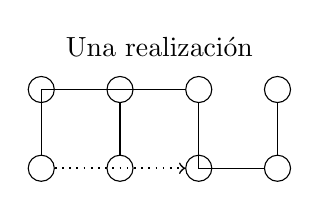
\begin{tikzpicture}[remember picture]
\pic (A) {array};
\path (A11) -- (A14) node[midway,above=3mm] {Una realización};
\draw[fluct] (A21)--(A23);
\end{tikzpicture}}
&
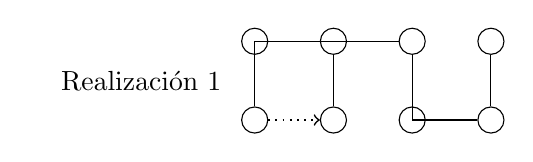
\begin{tikzpicture}[remember picture]
\pic (B) {array};
\path (B11) -- (B21) node[midway,left=3mm] (B_label) {Realización 1};
\draw[fluct] (B21)--(B22);
\node (R1) [left of = B_label, left=2mm] {};
\end{tikzpicture}
\\
&
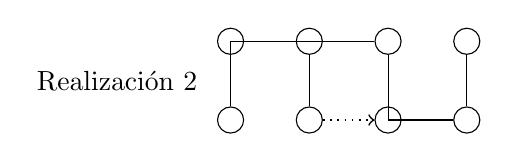
\begin{tikzpicture}[remember picture]
\pic (C) {array};
\path (C11) -- (C21) node[midway,left=3mm] {Realización 2};
\draw[fluct] (C22)--(C23);
\end{tikzpicture}
\\
&
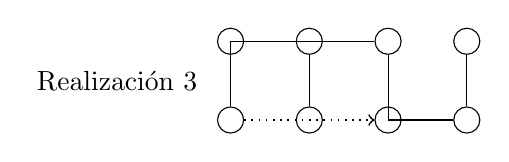
\begin{tikzpicture}[remember picture]
\pic (D) {array};
\path (D11) -- (D21) node[midway,left=3mm] {Realización 3};
\draw[fluct] (D21)--(D23);
\end{tikzpicture}
\\
&
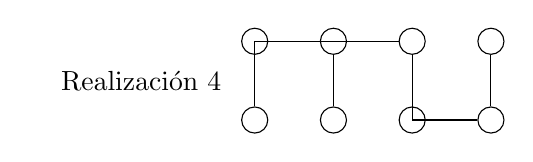
\begin{tikzpicture}[remember picture]
\pic (E) {array};
\path (E11) -- (E21) node[midway,left=3mm] (E_label) {Realización 4};
\node (R4) [left of = E_label, left=2mm] {};
\end{tikzpicture}
\end{tabular}

\tikz[remember picture, overlay] \draw[thick, dotted,->] (A14) + (3mm,2mm) -- (R1);
\tikz[remember picture, overlay] \draw[thick, dotted,->] (A24) + (3mm,-2mm) -- (R4);

\caption{Diferencia de realizaciones entre VPG (izquierda) y PG (derecha).}
\label{fig:realizaciones}
\end{figure}

Para intentar solucionar el problema se introdujo VPG-x que vuelve a muestrear cierta porción de los enlaces. Aunque se reduce la ganancia en tiempo computacional, aún así los resultados no llegan a ser iguales al PG en ciertas condiciones.

Para aplicar los algoritmos se necesita tener la descripción de una red y una o múltiples realizaciones sea el caso del algoritmo que se desee aplicar.

\section{Descripciones de red y realizaciones} \label{descripciones-realizaciones}
Para la creación de la \emph{descripción} de una red es simple: se debe decidir en esencia para cada uno de los enlaces presentes si es que este se considera fijo --siempre presente-- o fluctuante y el costo que incurre cada nodo en mantener cada enlace.

La forma esto se determina varía según la naturaleza de la red. Si la red se crea artificialmente, el costo se puede decidir arbitrariamente y los enlaces se pueden crear al azar decidiendo qué porcentaje de enlaces se quieren fijos con una variable $q_fix$ (a veces nombrado \emph{background}) y qué porcentaje fluctuantes con una variable $q_fluct$; obviamente esto nos deja que existe un porcentaje de enlaces que no están presentes $q_{miss} = 1-q_{fix}-q_{fluct}$.

Mientras que si lo que se quiere resolver es una proteína o compuesto físico, el tipo de enlace químico determina el tipo de enlace en la red y su costo.

Dada la naturaleza probabilística de los enlaces fluctuantes es necesario crear \emph{realizaciones}. Aunque la creación de una red es idéntica para los dos algoritmos, las realizaciones varían fundamentalmente entre PG y VPG. En PG se usan para establecer para cada enlace fluctuante si se encuentra presente o no. Para ello se debe decidir con qué probabilidad es que estos estén presentes en la red eligiendo un hiperparámetro $p$ tal que $0\leq p \leq 1$ que representa la fracción de los enlaces fluctuantes que están presentes en la red o, análogamente, el porcentaje de veces que cada enlace está presente en las múltiples realizaciones. En VPG mientras tanto se aproxima el comportamiento anterior asumiendo que los enlaces fluctuantes siempre están presentes pero cambiando su costo por $p*cost$.

Se puede apreciar que $p$ abstrae todo el ambiente en el que la red se encuentra. Todos los factores que permitan que haya más enlaces presentes o que por el contrario prevenga que los enlaces fluctuantes se encuentren presentes. Para una proteína puede representar la cantidad de energía que hay en el ambiente.

Según la descripción de una red dada en la figura \ref{fig:descripcion-red}, $p=0.5$ y $cost=5.0$ se puede crear las posibles instancias para PG que se muestra en la figura \ref{fig:instancias-pg} y para VPG en la figura \ref{fig:instancias-vpg}.

\begin{figure}
\centering
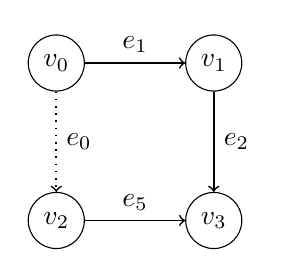
\begin{tikzpicture}[align=center,node distance=2cm]
\tikzstyle{vertex}=[circle,draw=black]
\tikzstyle{fixed}=[->,semithick]
\tikzstyle{fluct}=[->,semithick, dotted]

\node[vertex] (v0) {$v_0$};
\node[vertex] (v1) [right of = v0] {$v_1$};
\node[vertex] (v2) [below of = v0] {$v_2$};
\node[vertex] (v3) [right of = v2] {$v_3$};

\path[every node] 
  (v0) edge [fixed] node[auto] {$e_1$} (v1)
  (v0) edge [fluct] node[auto] {$e_0$} (v2)
  (v1) edge [fixed] node[auto] {$e_2$} (v3)
  (v2) edge [fixed] node[auto] {$e_5$} (v3);
\end{tikzpicture}
\caption{Descripción de una red. Los enlaces punteados son fluctuantes y los sólidos fijos.}
\label{fig:descripcion-red}
\end{figure}

\begin{figure}
\centering
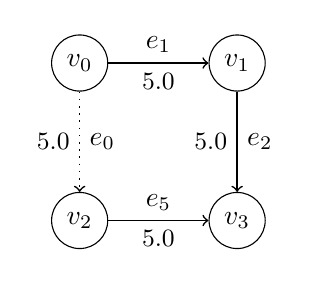
\begin{tikzpicture}[align=center,node distance=2cm]
\tikzstyle{vertex}=[circle,draw=black]
\tikzstyle{fixed}=[->,semithick]
\tikzstyle{fluct}=[->,semithick, dotted]

\node[vertex] (v0) {$v_0$};
\node[vertex] (v1) [right of = v0] {$v_1$};
\node[vertex] (v2) [below of = v0] {$v_2$};
\node[vertex] (v3) [right of = v2] {$v_3$};

\path[every node] 
  (v0) edge [fixed] node[auto, label={[font=\small]below:$5.0$}] {$e_1$} (v1)
  (v0) edge [fluct] node[auto, label={[font=\small]left:$5.0$}] {$e_0$} (v2)
  (v1) edge [fixed] node[auto, label={[font=\small]left:$5.0$}] {$e_2$} (v3)
  (v2) edge [fixed] node[auto, label={[font=\small]below:$5.0$}] {$e_5$} (v3);
\end{tikzpicture}
\qquad
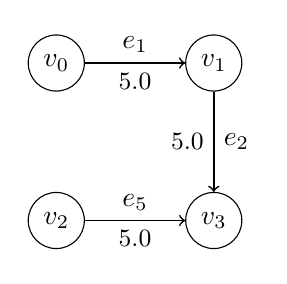
\begin{tikzpicture}[align=center,node distance=2cm]
\tikzstyle{vertex}=[circle,draw=black]
\tikzstyle{fixed}=[->,semithick]
\tikzstyle{fluct}=[->,semithick, dotted]

\node[vertex] (v0) {$v_0$};
\node[vertex] (v1) [right of = v0] {$v_1$};
\node[vertex] (v2) [below of = v0] {$v_2$};
\node[vertex] (v3) [right of = v2] {$v_3$};

\path[every node] 
  (v0) edge [fixed] node[auto, label={[font=\small]below:$5.0$}] {$e_1$} (v1)
  (v1) edge [fixed] node[auto, label={[font=\small]left:$5.0$}] {$e_2$} (v3)
  (v2) edge [fixed] node[auto, label={[font=\small]below:$5.0$}] {$e_5$} (v3);
\end{tikzpicture}
\caption{Diferentes instancias para PG}
\label{fig:instancias-pg}
\end{figure}

\begin{figure}
\centering
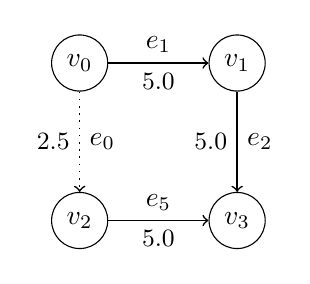
\begin{tikzpicture}[align=center,node distance=2cm]
\tikzstyle{vertex}=[circle,draw=black]
\tikzstyle{fixed}=[->,semithick]
\tikzstyle{fluct}=[->,semithick, dotted]

\node[vertex] (v0) {$v_0$};
\node[vertex] (v1) [right of = v0] {$v_1$};
\node[vertex] (v2) [below of = v0] {$v_2$};
\node[vertex] (v3) [right of = v2] {$v_3$};

\path[every node] 
  (v0) edge [fixed] node[auto, label={[font=\small]below:$5.0$}] {$e_1$} (v1)
  (v0) edge [fluct] node[auto, label={[font=\small]left:$2.5$}] {$e_0$} (v2)
  (v1) edge [fixed] node[auto, label={[font=\small]left:$5.0$}] {$e_2$} (v3)
  (v2) edge [fixed] node[auto, label={[font=\small]below:$5.0$}] {$e_5$} (v3);
\end{tikzpicture}
\caption{Una única instancia para VPG}
\label{fig:instancias-vpg}
\end{figure}

\section{Descripción general de PG y VPG} \label{descripcion-general}
González\parencite{Gonzalez2011} explica los algoritmos de la siguiente manera: considérese una red consistente de vértices ${V_n}, n=1,2,\ldots,N$, con una lista de aristas ${e_m}, m=1,2,\ldots,M$. La capacidad del enlace $m$-ésimo se denota por $e_m$. El algoritmo PG y VPG siguen los siguientes procedimientos y operaciones:

\begin{enumerate}
	\item Inicialice el grafo con un conjunto de vértices aislados con 6 grados de libertad (\emph{Degres Of Freedom} o \emph{DOF}) cada vértice $v_n$ siendo 6,
	\item De la lista de enlaces ${e_m}$, insertar el eje $e_k$ con la capacidad $c_k$ en el grafo. Sea $v_i$ y $v_j$ los dos vértices incidentes para el eje $e_k$.
	\item Recopilar 6 \emph{pebbles} para el vértice $v_i$ haciendo una búsqueda por amplitud. La teoría de grafos en la que se basan los algoritmos garantiza que esta búsqueda será exitosa debido a que esos 6 \emph{pebbles} representan los 6 grados de libertad de la red misma
	\item Marcar el vértice {$v_i$} cómo visitado, intentar recolectar $c_k$ \emph{pebbles} haciendo una búsqueda por amplitud manteniendo los 6 \emph{pebbles} sin utilizar. Si no se pueden completar $c_k$ \emph{pebbles} en un intento, continuar intentando hasta que haya suficientes \emph{pebbles} libres en $v_j$ para cubrir el eje $e_k$, o si no hay suficientes \emph{pebbles} hacer una búsqueda fallida.
	\item Si se recolectan $c_k$ o más \emph{pebbles} en el vértice $v_j$, cubrir el enlace $e_k$ con $c_k$ \emph{pebbles}. Si no, todos los vértices visitados en la búsqueda fallida se condensan en un sólo vértice. Si ${e_m}$ no está vacía ir al paso 2.
	\item Fin de VPG
\end{enumerate}


\begin{figure}
\centering
\begin{subfigure}{0.30\textwidth}
\begin{tikzpicture}[align=center,node distance=2cm]
\tikzstyle{vertex}=[circle,draw=black]
\tikzstyle{fixed}=[-,semithick]

\node[vertex] (v0) {$v_0$};
\node[vertex] (v1) [right of = v0] {$v_1$};
\node[vertex] (v2) [below of = v0] {$v_2$};
\node[vertex] (v3) [right of = v2] {$v_3$};

\node[left =  0mm of v0] (v0_dof) {6};
\node[right = 0mm of v1] (v1_dof) {6};
\node[left =  0mm of v2] (v2_dof) {6};
\node[right = 0mm of v3] (v3_dof) {6};

\end{tikzpicture}
\caption{}
\end{subfigure}
\hfill
\begin{subfigure}{0.30\textwidth}
\begin{tikzpicture}[align=center,node distance=2cm]
\tikzstyle{vertex}=[circle,draw=black]
\tikzstyle{fixed}=[-,semithick]

\node[vertex] (v0) {$v_0$};
\node[vertex] (v1) [right of = v0] {$v_1$};
\node[vertex] (v2) [below of = v0] {$v_2$};
\node[vertex] (v3) [right of = v2] {$v_3$};

\node[left =  0mm of v0] (v0_dof) {6};
\node[right = 0mm of v1] (v1_dof) {3};
\node[left =  0mm of v2] (v2_dof) {6};
\node[right = 0mm of v3] (v3_dof) {3};

\path
  (v0) edge [fixed] node[very near end, auto] {$3$} (v1)
  (v2) edge [fixed] node[very near end, auto] {$3$} (v3);
\end{tikzpicture}
\caption{}
\end{subfigure}
\hfill
\begin{subfigure}{0.30\textwidth}
\begin{tikzpicture}[align=center,node distance=2cm]
\tikzstyle{vertex}=[circle,draw=black]
\tikzstyle{fixed}=[-,semithick]

\node[vertex] (v0) {$v_0$};
\node[vertex] (v1) [right of = v0] {$v_1$};
\node[vertex] (v2) [below of = v0] {$v_2$};
\node[vertex, very thick] (v3) [right of = v2] {$v_3$};

\node[left =  0mm of v0] (v0_dof) {6};
\node[right = 0mm of v1] (v1_dof) {3};
\node[left =  0mm of v2] (v2_dof) {3};
\node[right = 0mm of v3] (v3_dof) {6};

\path
  (v0) edge [fixed] node[very near end, auto] {$3$} (v1)
  (v2) edge [fixed] node[very near start, auto] {$3$} node[very near end, auto] (v3left) {} (v3)
  (v3) edge[dashed] node[midway, right] {$7$} (v1);

\draw[->]	($(v2_dof.north) + (1mm,2mm)$) arc [start angle = 140, end angle = 55, radius = 0.65cm];
\draw[->]	($(v3left.south) + (-1mm,-3mm)$) arc [start angle = 190, end angle = 335, radius = 0.65cm];
\end{tikzpicture}
\caption{}
\end{subfigure}
\\
\begin{subfigure}{0.30\textwidth}
\begin{tikzpicture}[align=center,node distance=2cm]
\tikzstyle{vertex}=[circle,draw=black]
\tikzstyle{fixed}=[-,semithick]

\node[vertex] (v0) {$v_0$};
\node[vertex] (v1) [right of = v0] {$v_1$};
\node[vertex] (v2) [below of = v0] {$v_2$};
\node[vertex, very thick] (v3) [right of = v2] {$v_3$};

\node[left =  0mm of v0] (v0_dof) {3};
\node[right = 0mm of v1] (v1_dof) {6};
\node[left =  0mm of v2] (v2_dof) {3};
\node[right = 0mm of v3] (v3_dof) {6};

\path
  (v0) edge [fixed] node[very near start, auto] {$3$} node[very near end, auto] (v1left) {} (v1)
  (v2) edge [fixed] node[very near start, auto] {$3$} (v3)
  (v3) edge[dashed] node[midway, right] {$7$} (v1);

\draw[->]	($(v0_dof.north) + (1mm,2mm)$) arc [start angle = 140, end angle = 55, radius = 0.65cm];
\draw[->]	($(v1left.north) + (1mm,2mm)$) arc [start angle = 140, end angle = 40, radius = 0.65cm];
\end{tikzpicture}
\caption{}
\end{subfigure}
\hfill
\begin{subfigure}{0.30\textwidth}
\begin{tikzpicture}[align=center,node distance=2cm]
\tikzstyle{vertex}=[circle,draw=black]
\tikzstyle{fixed}=[-,semithick]

\node[vertex] (v0) {$v_0$};
\node[vertex] (v1) [right of = v0] {$v_1$};
\node[vertex] (v2) [below of = v0] {$v_2$};
\node[vertex, very thick] (v3) [right of = v2] {$v_3$};

\node[left =  0mm of v0] (v0_dof) {3};
\node[right = 0mm of v1] (v1_dof) {6};
\node[left =  0mm of v2] (v2_dof) {3};
\node[right = 0mm of v3] (v3_dof) {6};

\path
  (v0) edge [fixed] node[very near start, auto] {$3$} node[very near end, auto] (v1left) {} (v1)
  (v2) edge [fixed] node[very near start, auto] {$3$} (v3)
  (v3) edge [fixed] node[midway, right] {$6$} (v1);

\node[draw, dashed, inner sep = 2mm, fit = (v1) (v1_dof) (v3) (v3_dof)] (cover) {};
\node[above = 1 mm of cover] {Clúster rígido};
\end{tikzpicture}
\caption{}
\end{subfigure}
\hfill
\begin{subfigure}{0.30\textwidth}
\begin{tikzpicture}[align=center,node distance=2cm]
\tikzstyle{vertex}=[circle,draw=black]
\tikzstyle{fixed}=[-,semithick]

\node[vertex] (v0) {$v_0$};
\node (v1_) [right of = v0] {};
\node[vertex] (v2) [below of = v0] {$v_2$};
\node (v3_) [right of = v2] {};

\path (v1_) -- (v3_) node[vertex, midway] (v1) {$v_1$};

\node[left =  0mm of v0] (v0_dof) {3};
\node[right = 0mm of v1] (v1_dof) {6};
\node[left =  0mm of v2] (v2_dof) {3};

\path
  (v0) edge [fixed] node[very near start, auto] {$3$} (v1)
  (v2) edge [fixed] node[near start, below] {$3$} (v1);
\end{tikzpicture}
\caption{}
\end{subfigure}
\caption{Ejemplo de aplicar VPG a 4 nodos.}
\label{fig:ejemplo-vpg}
\end{figure}

En la figura \ref{fig:ejemplo-vpg} se muestra un ejemplo de aplicar el algoritmo VPG a una simple red. Una línea punteada denota el enlace que se está agregando a la red en ese paso: (a)  estado inicial de la red; (b) se agregan 2 enlaces de $v_1$ a $v_0$ y de $v_3$ a $v_2$; (c) se quiere agregar un nuevo enlace de $v_1$ a $v_3$ con un costo de 7, $v_3$ solicita \emph{pebbles} a $v_2$; (d) $v_1$ solicita los 3 \emph{pebbles} que gastó para el enlace con $v_0$, se hace el \emph{backtrack}; (e) se han acarreado todos los \emph{pebbles} que disponibles para $v_1$ y $v_3$ pero aún así no se completa el nuevo enlace, éste se hace con los \emph{pebbles} que se obtuvieron y se identifica la región como un clúster rígido; (f) se condensa el clúster en un sólo vértice.

\section{Clusters rígidos y colapso} \label{cluster-rigido}

Los clúster rígidos, también informalmente llamados subgrafos de Lemann, son aquellas partes de la red en las que solamente se tienen disponibles los grados de libertad triviales de la red en sí misma (6 para 3 dismensiones), y todos los enlaces salientes de los vértices se apuntan entre sí. Los clúster rígidos representan secciones de la red que se comportan como un cuerpo sólido. Están unidos a la red mediante enlaces que están cubiertos por vértices fuera del clúster y no tienen enlaces salientes. La figura \ref{fig:cluster-rigido} muestra un cluster rígido. 

\begin{figure}
\centering
\begin{tikzpicture}[align=center,node distance=2cm]
\tikzstyle{vertex}=[circle,draw=black]
\tikzstyle{fixed}=[-,semithick]

\node[vertex] (v0) {$v_0$};
\node[vertex, very thick] (v1) [right of = v0] {$v_1$};
\node[vertex] (v2) [right of = v1] {$v_2$};
\node[vertex] (v3) [below of = v1] {$v_3$};
\node[vertex] (v4) [right of = v3] {$v_4$};

\path
  (v0) edge [fixed] node[very near start, auto] {$5$} (v1)
  (v1) edge [fixed] node[very near end, auto] {$4$} (v2)
  (v1) edge [fixed] node[very near end, auto] {$4$} (v3)
  (v2) edge [fixed] node[very near start, auto] {$5$} (v4)
  (v3) edge [fixed] node[very near end, auto] {$5$} (v4);

\node[above = 0mm of v1] (v1_dof) {6};
\node[draw, dashed, inner sep = 2mm, fit = (v1_dof) (v1) (v2) (v3) (v4)] (cover) {};
\node[above = 1 mm of cover] {Clúster rígido};

\end{tikzpicture}
\caption{Ejemplo de un clúster rígido en 3 dimensiones}{$V_1$ tiene los 6 \emph{pebbles} de la red y se encuentra bloqueado. No hay más \emph{pebbles} disponibles.}
\label{fig:cluster-rigido}
\end{figure}

Cuándo se ha encontrado un clúster rígido, este se puede colapsar en un sólo vértice que representa todos los vértices que pertenecen al clúster rígido. La figura \ref{fig:ejemplo-vpg} muestra un ejemplo de condensación.

El objetivo principal de la condenzación es reducir el costo computacional de procesar la red. El condenzar todos los vértices en uno solo en representación de todos los demás permite visitar menos vértices dentro de la red al buscar \emph{pebbles} disponibles y reducir así la complejidad del algoritmo. Por otra parte la justificación teórica de la condensación es que esta no cambia la cantidad de grados de libertad final presentes en la red, solamente su distribución; y si solamente hay una cantidad mínima de \emph{pebbles} libres en la red, esto significa que toda la red es rígida y esos 6 \emph{pebbles} representan la libertad del conjunto en sí.

La implementación del colapso es importante y un poco delicada. Una implementación ingenua no mantiene la integridad de la red o podría tener una complejidad de $O(n^2)$. La implementación que se presenta en la sección \ref{vpg-paso-paso} es simple, intuitiva y mantiene el costo computacional en el orden de $O(n)$.

\section{Notación O-grande} \label{o-grande}
La notación O-grande se utiliza en el análisis de algoritmos para describir el desempeño de un procedimiento en memoria o en tiempo en el peor de los casos. El objetivo simplemente es describir que una función $f(x)$ en el peor de los casos siempre se desempeñará mejor que una función $M*g(x)$ para una $M$ específica y entradas de $x$ suficientemente grandes.

Formalmente se dice que una función $f(x) =  M*O(g(x)) as x \to \infty$  si y sólo si existe una constante positiva $M$ tal que para valores suficientemente grandes de $x$, el valor absoluto de $f(x)$ es a lo más M multiplicado por el valor absoluto de $g(X)$. Es decir,   $f(x) = O(g(x))$ si y sólo si existen números $M \in \mathbb{R} | M > 0	$ y $x_0 \in \mathbb{R}$ tal que \[|f(x)| \leq M|g(x)| \forall x \geq x_0 \]

Usualmente simplemente expresado como $f(x) = O(g(x))$ o utilizando la notación O como el conjunto de funciones que son cubiertas por $g(x)$ simplemente $f(x) \in O(g(x))$.

La relación anterior se expresa gráficamente en la figura \ref{fig:o-grande}.

Es importante recalcar que la notación O-grande no debe de utilizarse para representar la velocidad de un algoritmo sino solamente crecimiento de la complejidad conforme la entrada crece. Después de todo las constantes que se dejan implícitas pueden ser muy grandes por lo que aún un algoritmo considerado de alta complejidad, digamos \emph{bubble sort} que es $O(n^2)$, puede ser más rápido que uno de baja complejidad cómo \emph{merge sort} con $O(log\,n)$ para $n$ suficientemente pequeñas.

\begin{figure}
\centering
\begin{tikzpicture}
\begin{axis}[ticks = none, xmin=0, xmax=4, axis lines=left]
  \addplot[blue, thick, samples=100] (x,x*x + 2*x)
		node[below, yshift=-3mm, pos=0.75] {$f(x)$};
  \addplot[red, thick, samples=100] (x,2*x*x) node[left, pos=0.75] {$cg(x)$};
  \node at (axis cs:2,0) (origen) {};
  \draw [densely dotted] (axis cs:2,8) -- (axis cs:2,0);
\end{axis}
\node [below = 0cm of origen] {$x_0$};
\end{tikzpicture}
%TODO agregar x_0, quitar valores axis, acis de libro
\caption{Descripción gráfica de la notación O-grande}
\label{fig:o-grande}
\end{figure}

\section{Matrices dispersas} \label{matrices-dispersas}
Las matrices dispersas son aquellas matrices usualmente de gran tamaño pero que tienen la mayor parte de sus coeficientes en 0 y que por tanto una representación ingenua desperdicia mucha memoria para elementos redundantes. Para el manejo de éste caso particular se han diseñado representaciones adecuadas que minimizan la cantidad de memoria desperdiciada mientras que mantienen la semántica de una matriz común.

El uso de este tipo de técnicas permite hacer frente a problemas que serían intractables en memoria por la enorme cantidad de coeficientes en cero y al mismo tiempo ayuda a mejorar el desempeño en los problemas que son tractables pero que tienen un costo de memoria muy alto debido a que estas técnicas mejoran la localidad del programa.

Existen múltiples técnicas para representar una matriz dispersa, cada una de ellas con diferentes propiedades. De todas las representaciones la más popular es la que almacena en formato \emph{Compressed Storage Row} (CSR).  El formato CSR consta de tres componentes que describen a la matriz:

\begin{itemize}
  \item Un vector de punto flotante de tamaño $k$ en el que se almacenan los valores de los coeficientes.
  \item Un vector de tamaño $k$ en el que se almacenan los números de columna de los elementos distintos de 0.
  \item Un vector de tamaño $n+1$ siendo $n$ la cantidad de filas de la matriz en el cual se almacena la posición de la primera ocurrencia de cada fila.
\end{itemize}

Las diferentes representaciones tienen diferentes características de costo de acceso y de memoria pero es suficiente saber que el utilizar una matriz dispersa en el contexto adecuado permite mejorar enormemente el desempeño de un programa.